\section{Results}
\label{sec:Results}

\subsection{Simulated Geometries}

The simulated count for the detector designs is shown in Figure ~\ref{fig:SimCountRate}.
Not that this value does not include the scaling necessary to acheive the gamma discrimination. 
\begin{figure}
    \centering
    \begin{subfigure}[b]{0.45\textwidth}
        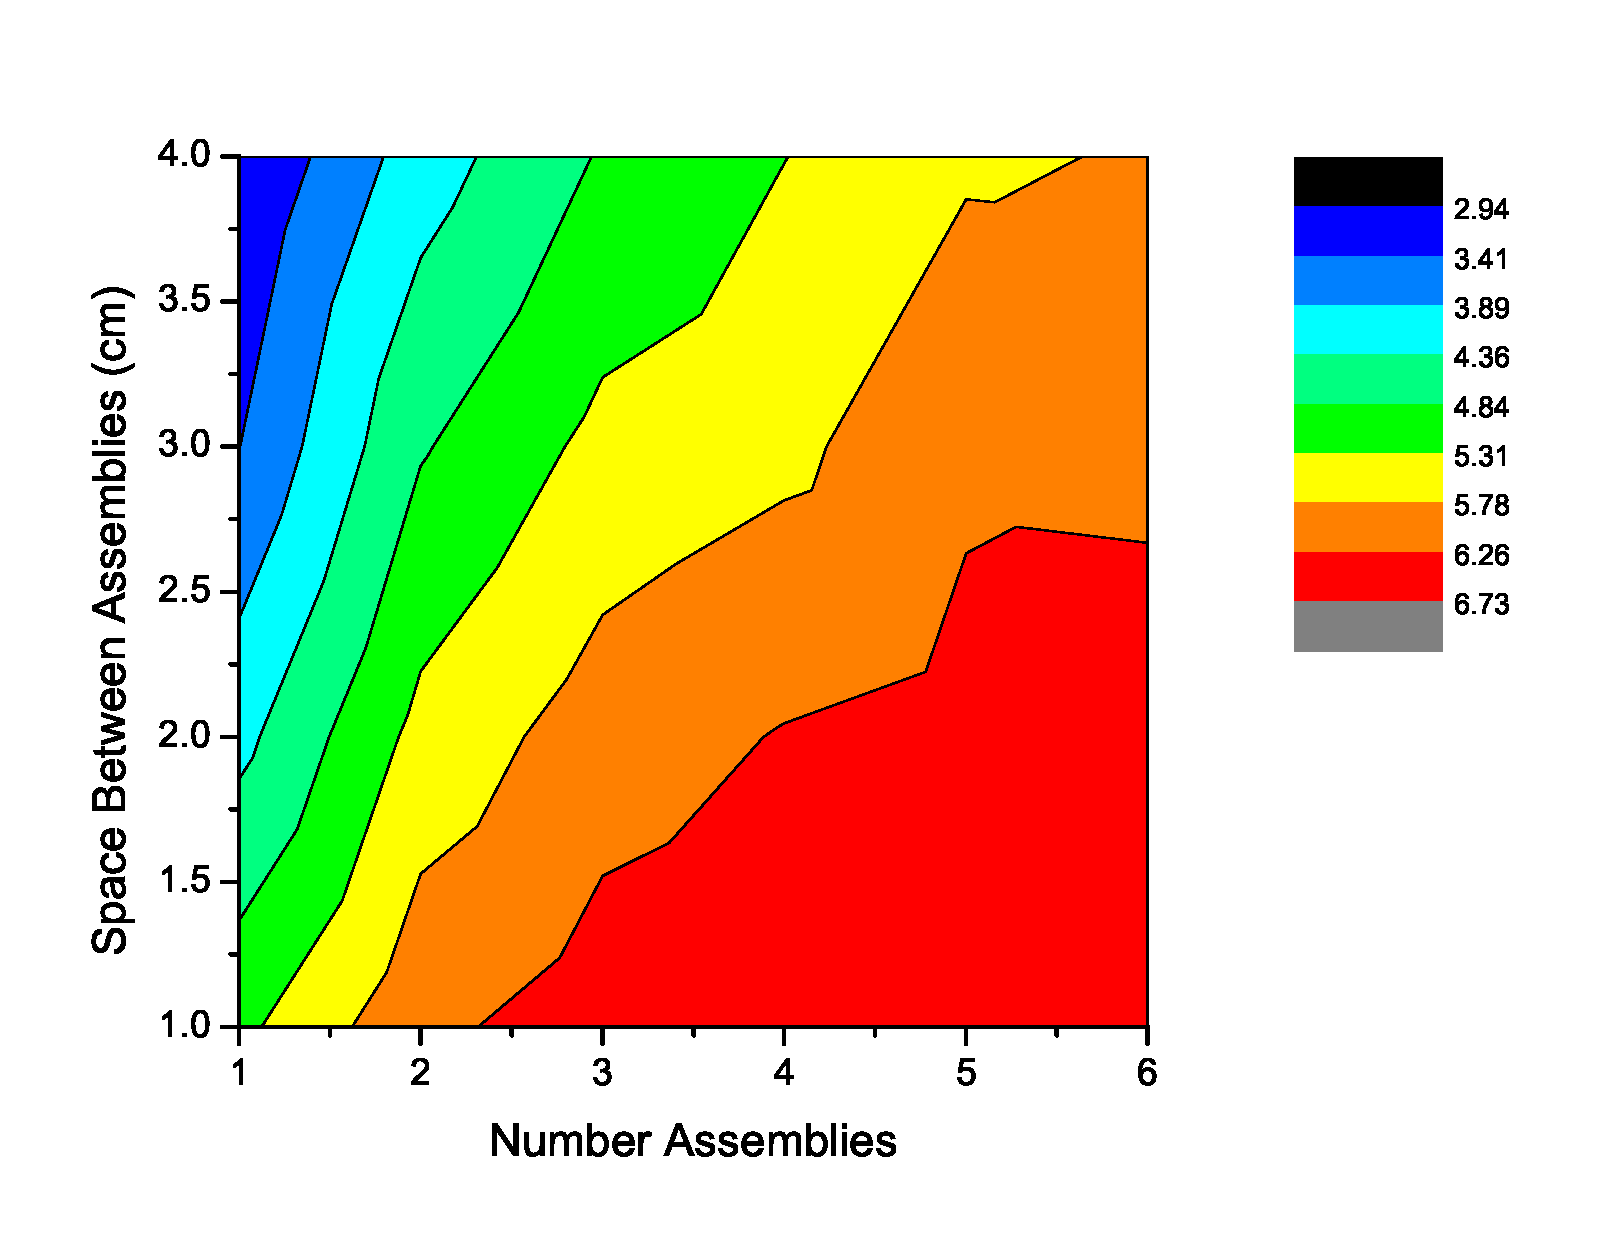
\includegraphics[width=\textwidth]{RPM8Opt_CR.eps}
        \caption{Count Rate per \SI{\per\nano\gram\iso[252]{Cf}}}
    \end{subfigure}%
    ~
    \begin{subfigure}[b]{0.45\textwidth}
        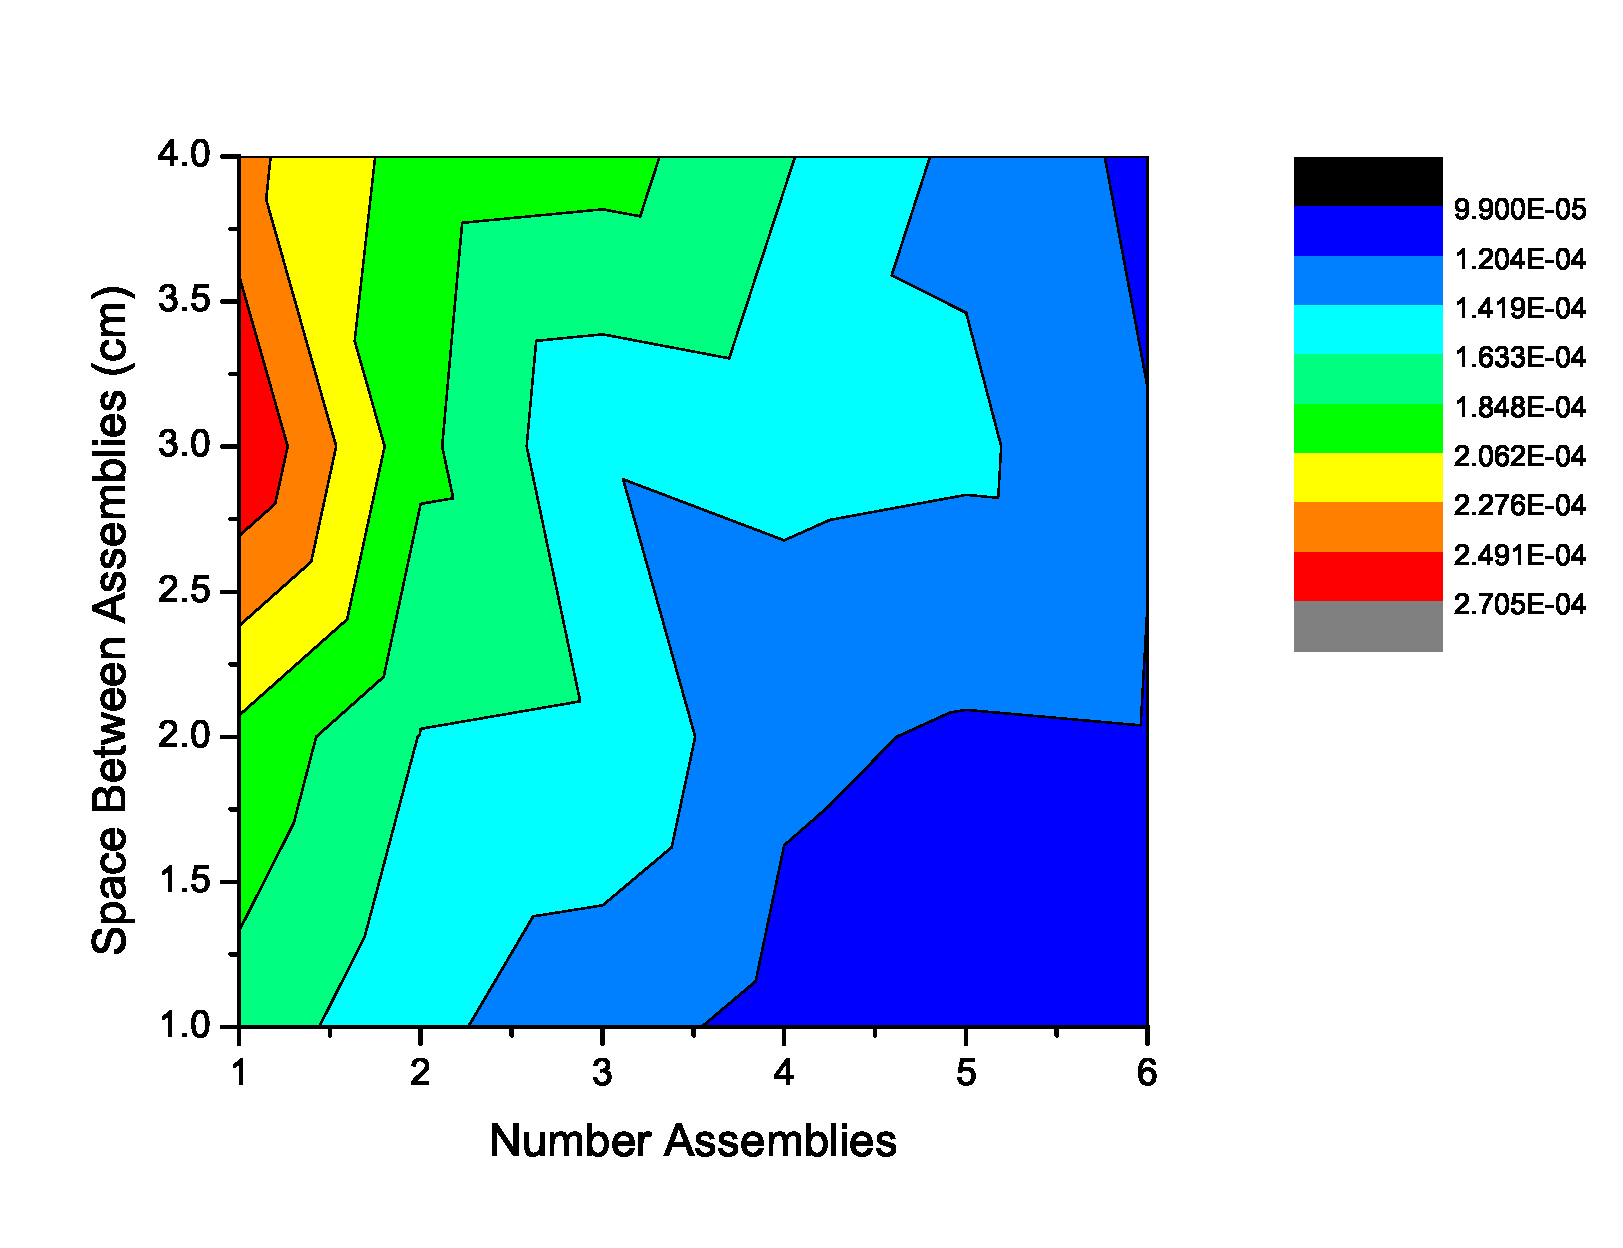
\includegraphics[width=\textwidth]{RPM8Opt_CRperLi.eps}
        \caption{Count Rate per nano gram \iso[252]{Cf} per \SI{\milli\gram} \iso[6]{Li}}
    \end{subfigure}
    \caption{Count rate per depdenance on number of assemblies and spacing of the simulated detectors. The amount of \iso[6]{Li} is not constnat}
    \label{fig:SimCountRate}
\end{figure}

\begin{figure}
	\centering
	\begin{subfigure}[b]{0.43\textwidth}
		\centering
		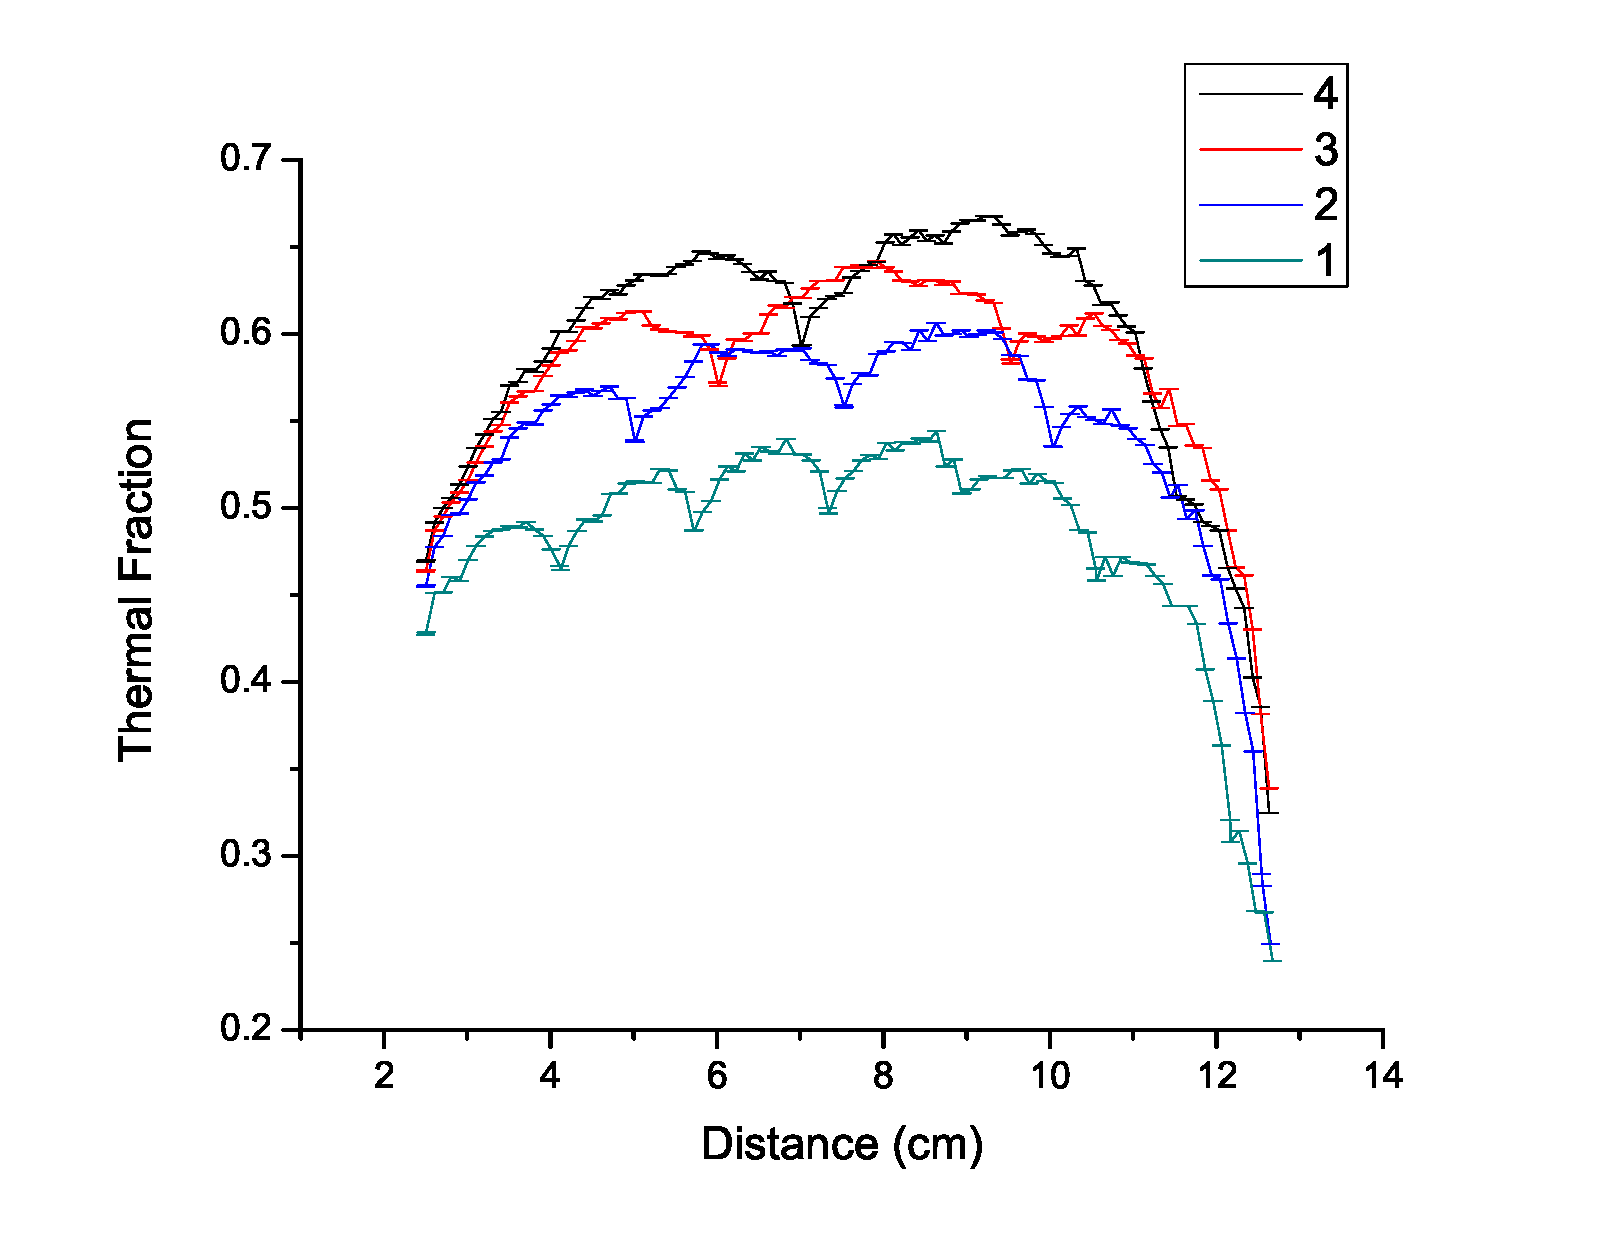
\includegraphics[width=\textwidth]{RPM8Opt_TF_1Assm.eps}
    \caption{1 Films per Assembly}
	\end{subfigure}%
	~
	\begin{subfigure}[b]{0.43\textwidth}
		\centering
		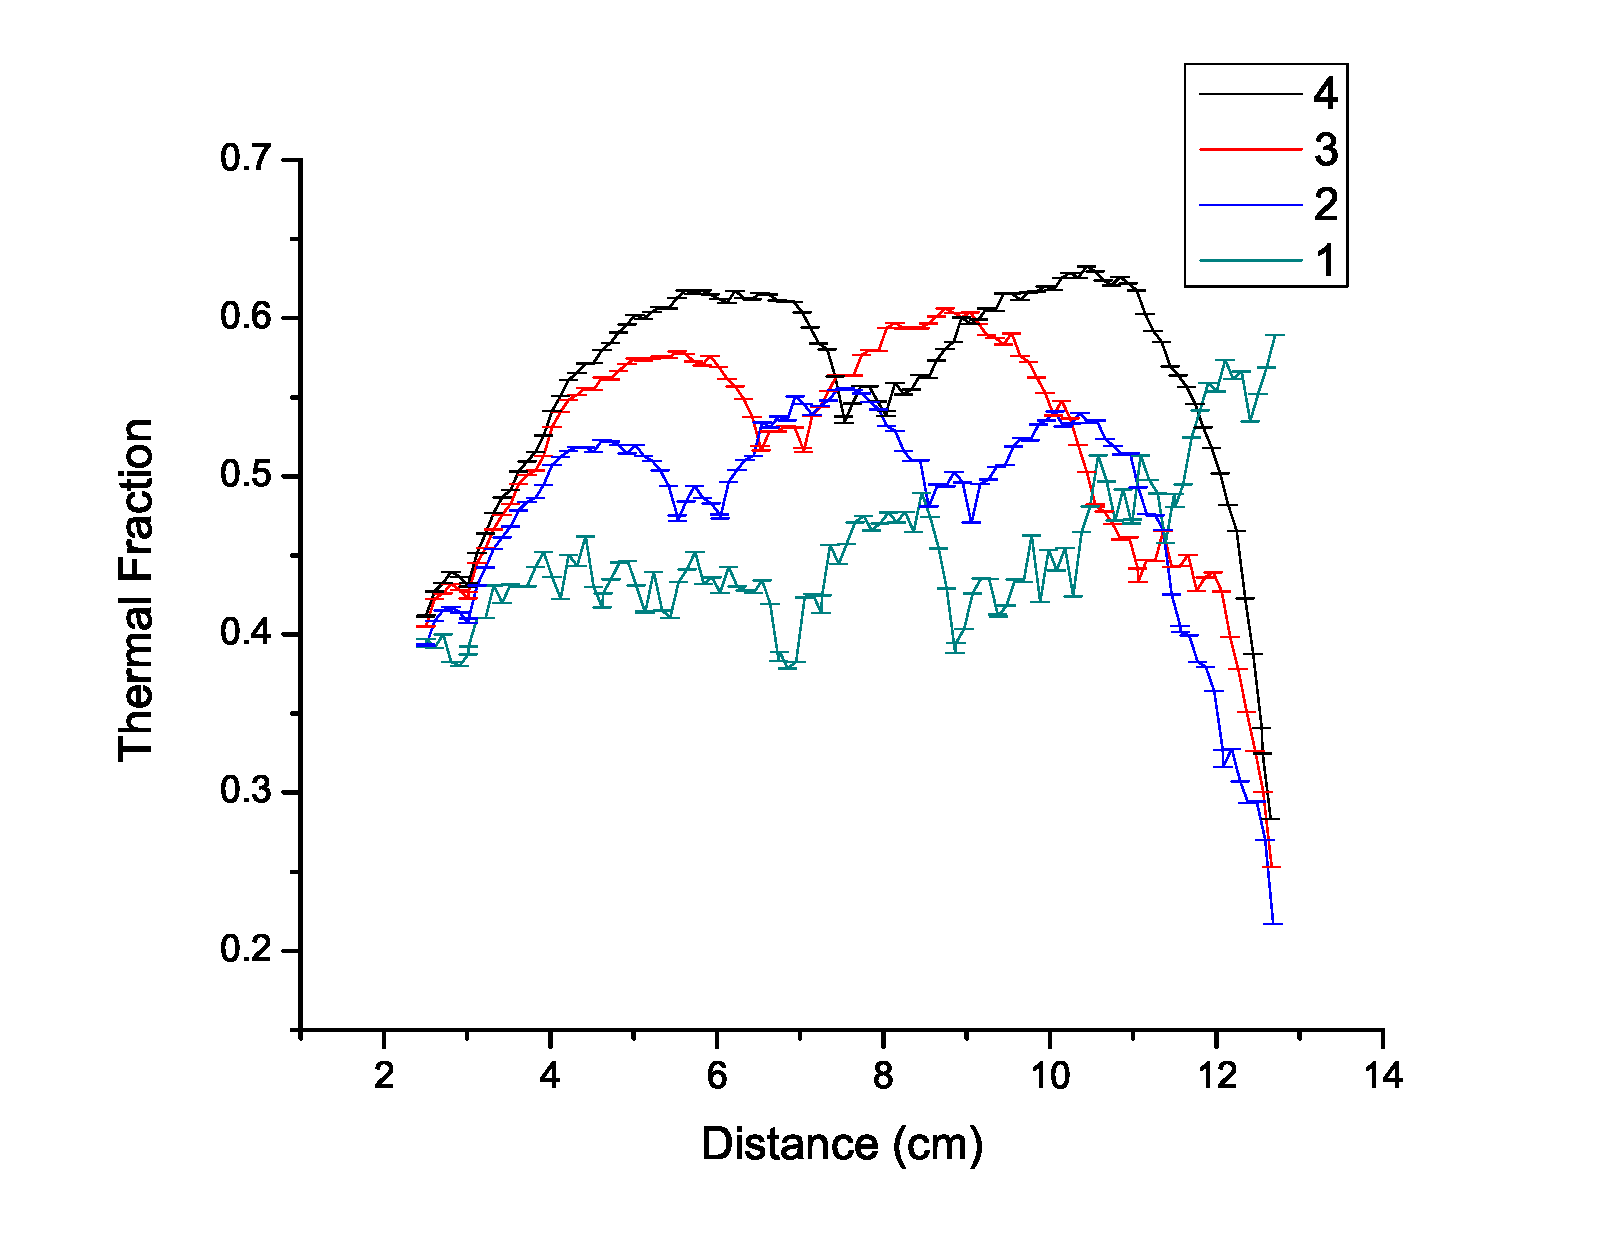
\includegraphics[width=\textwidth]{RPM8Opt_TF_2Assm.eps}
    \caption{2 Films per Assembly}
	\end{subfigure}	
	
  \begin{subfigure}[b]{0.43\textwidth}
		\centering
		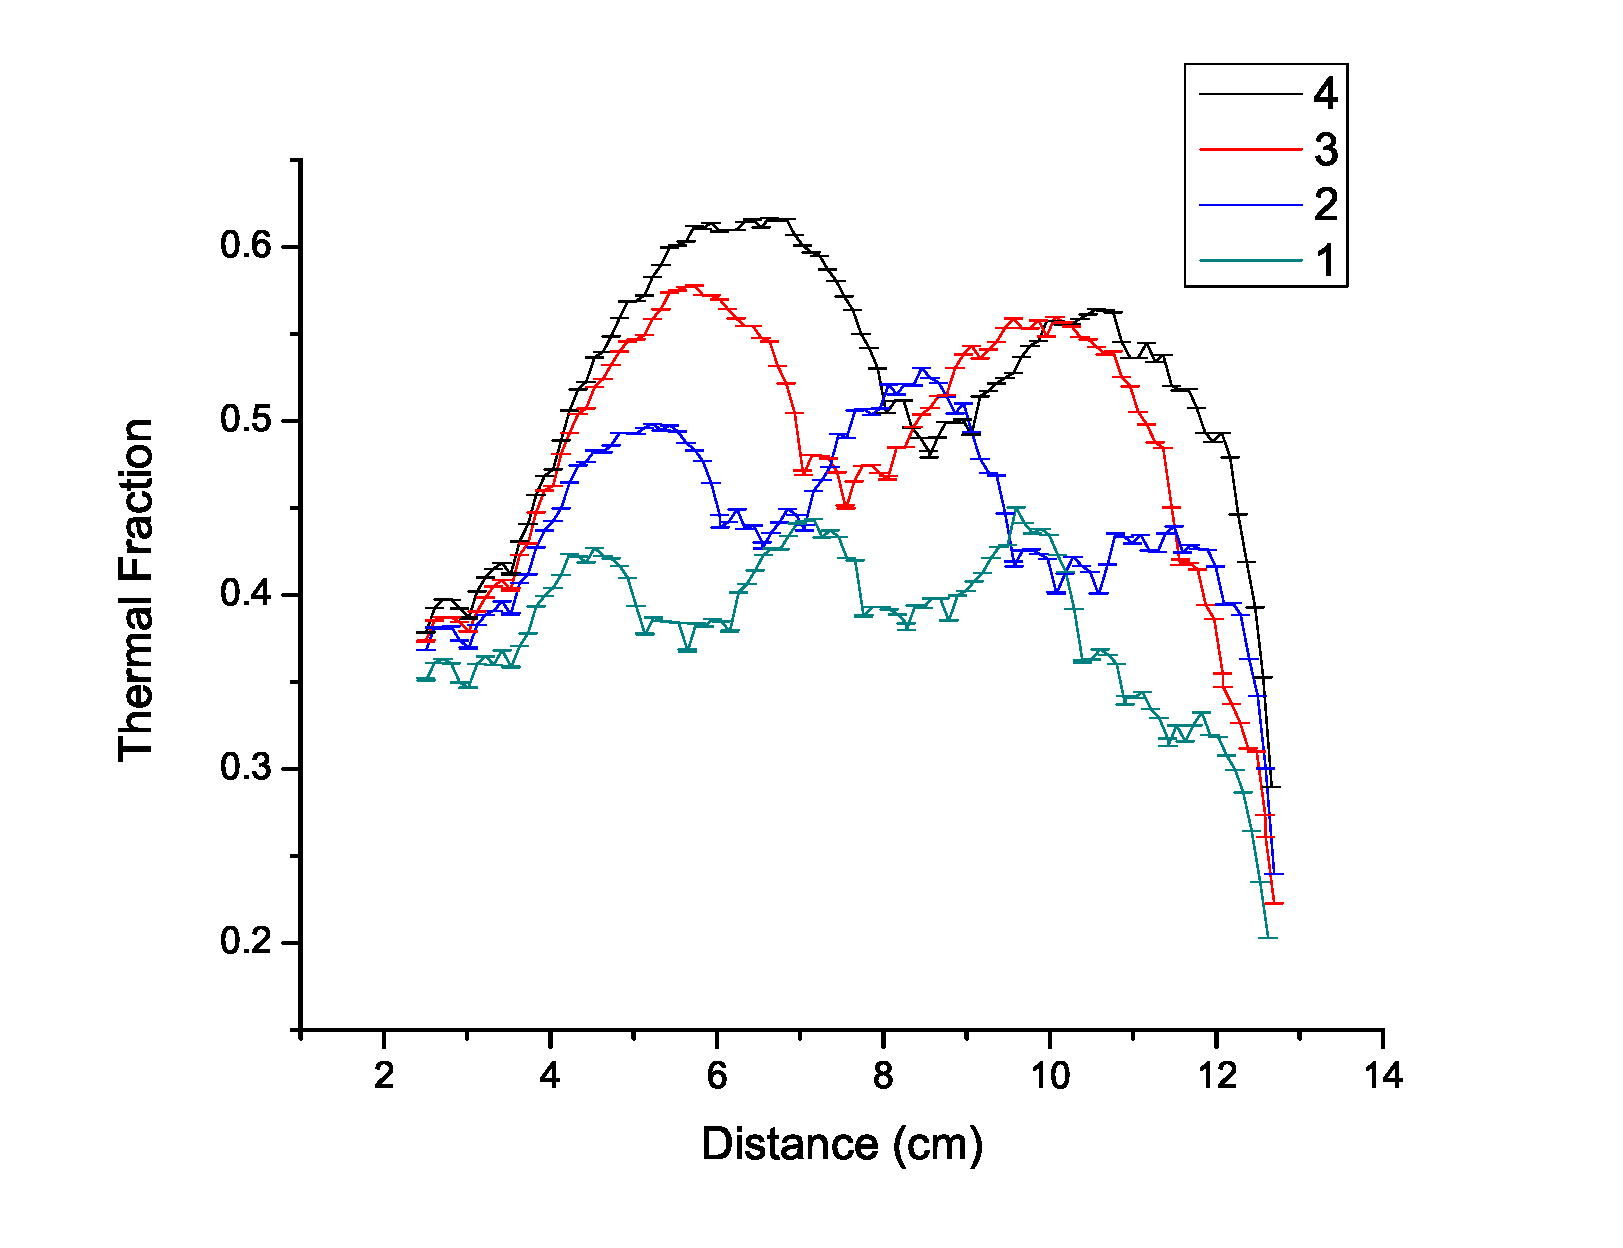
\includegraphics[width=\textwidth]{RPM8Opt_TF_3Assm.eps}
    \caption{3 Films per Assembly}
	\end{subfigure}%
	~
	\begin{subfigure}[b]{0.43\textwidth}
		\centering
		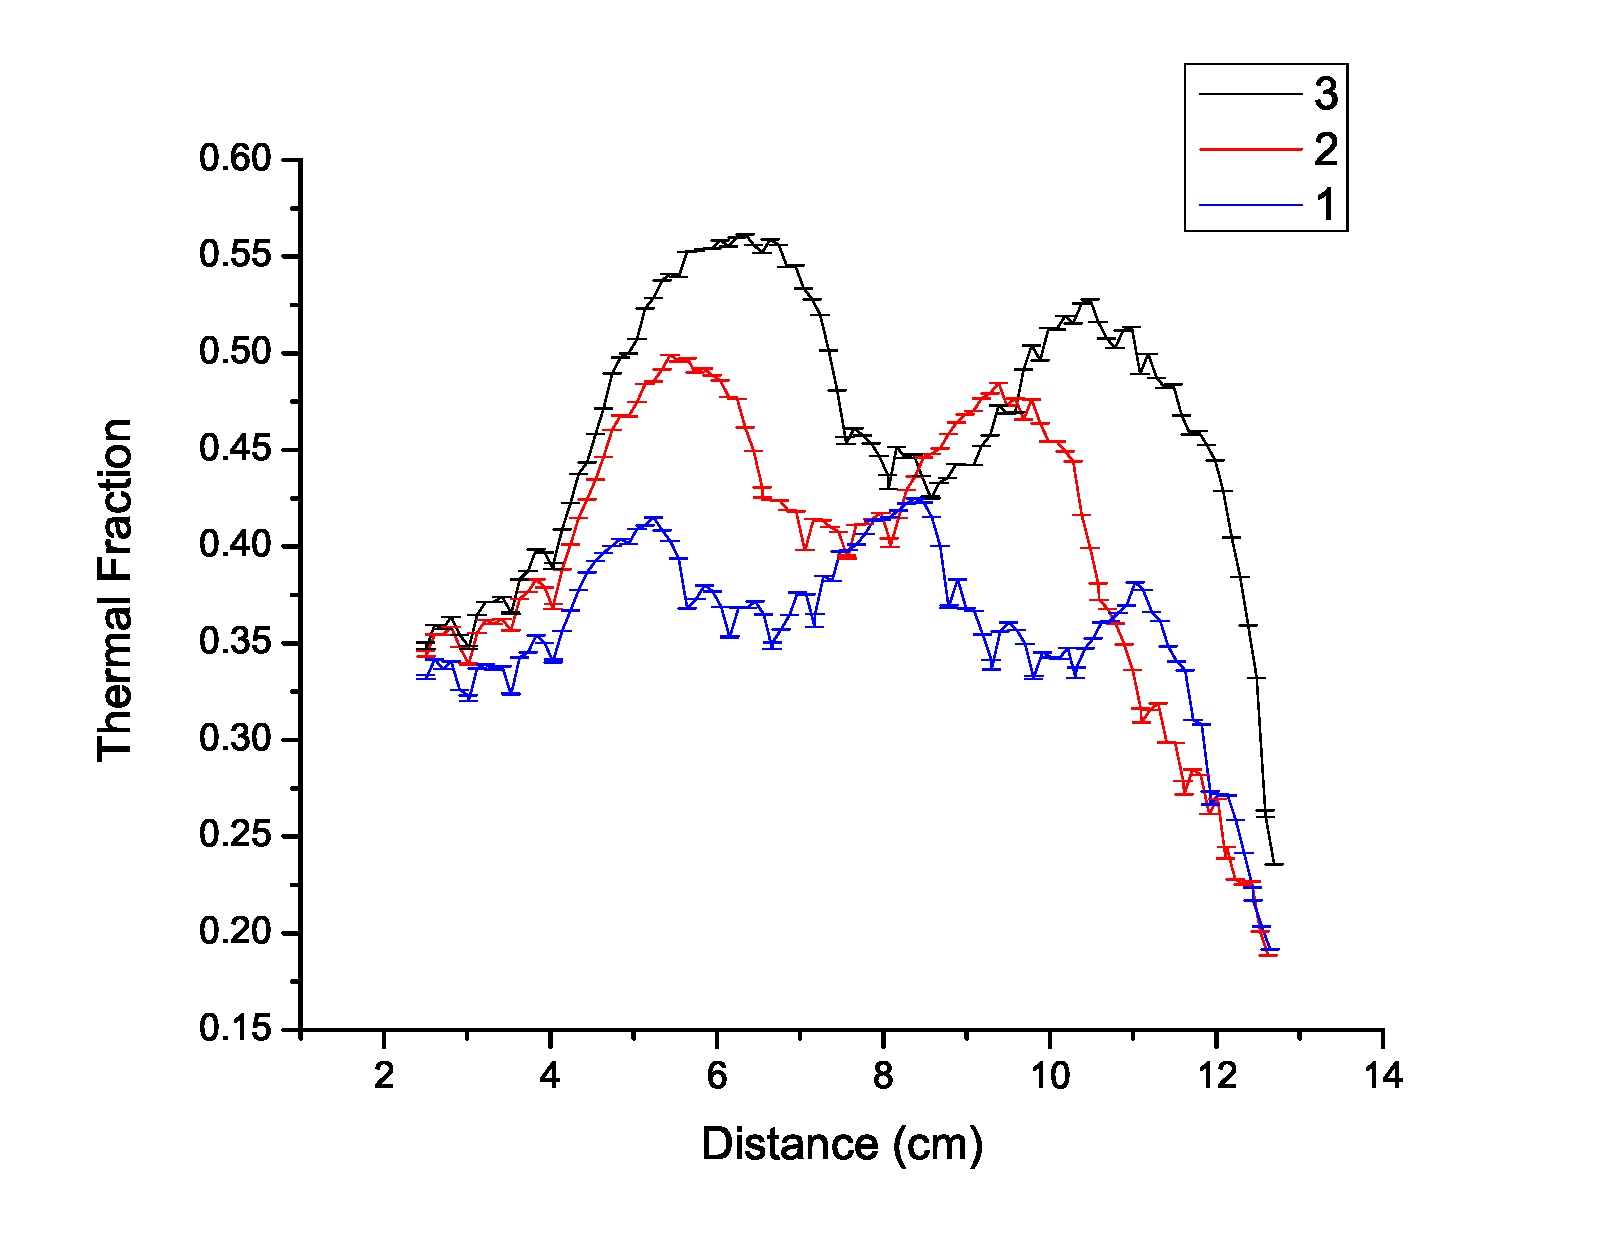
\includegraphics[width=\textwidth]{RPM8Opt_TF_4Assm.eps}
    \caption{4 Films per Assembly}
	\end{subfigure}	

	\begin{subfigure}[b]{0.43\textwidth}
		\centering
		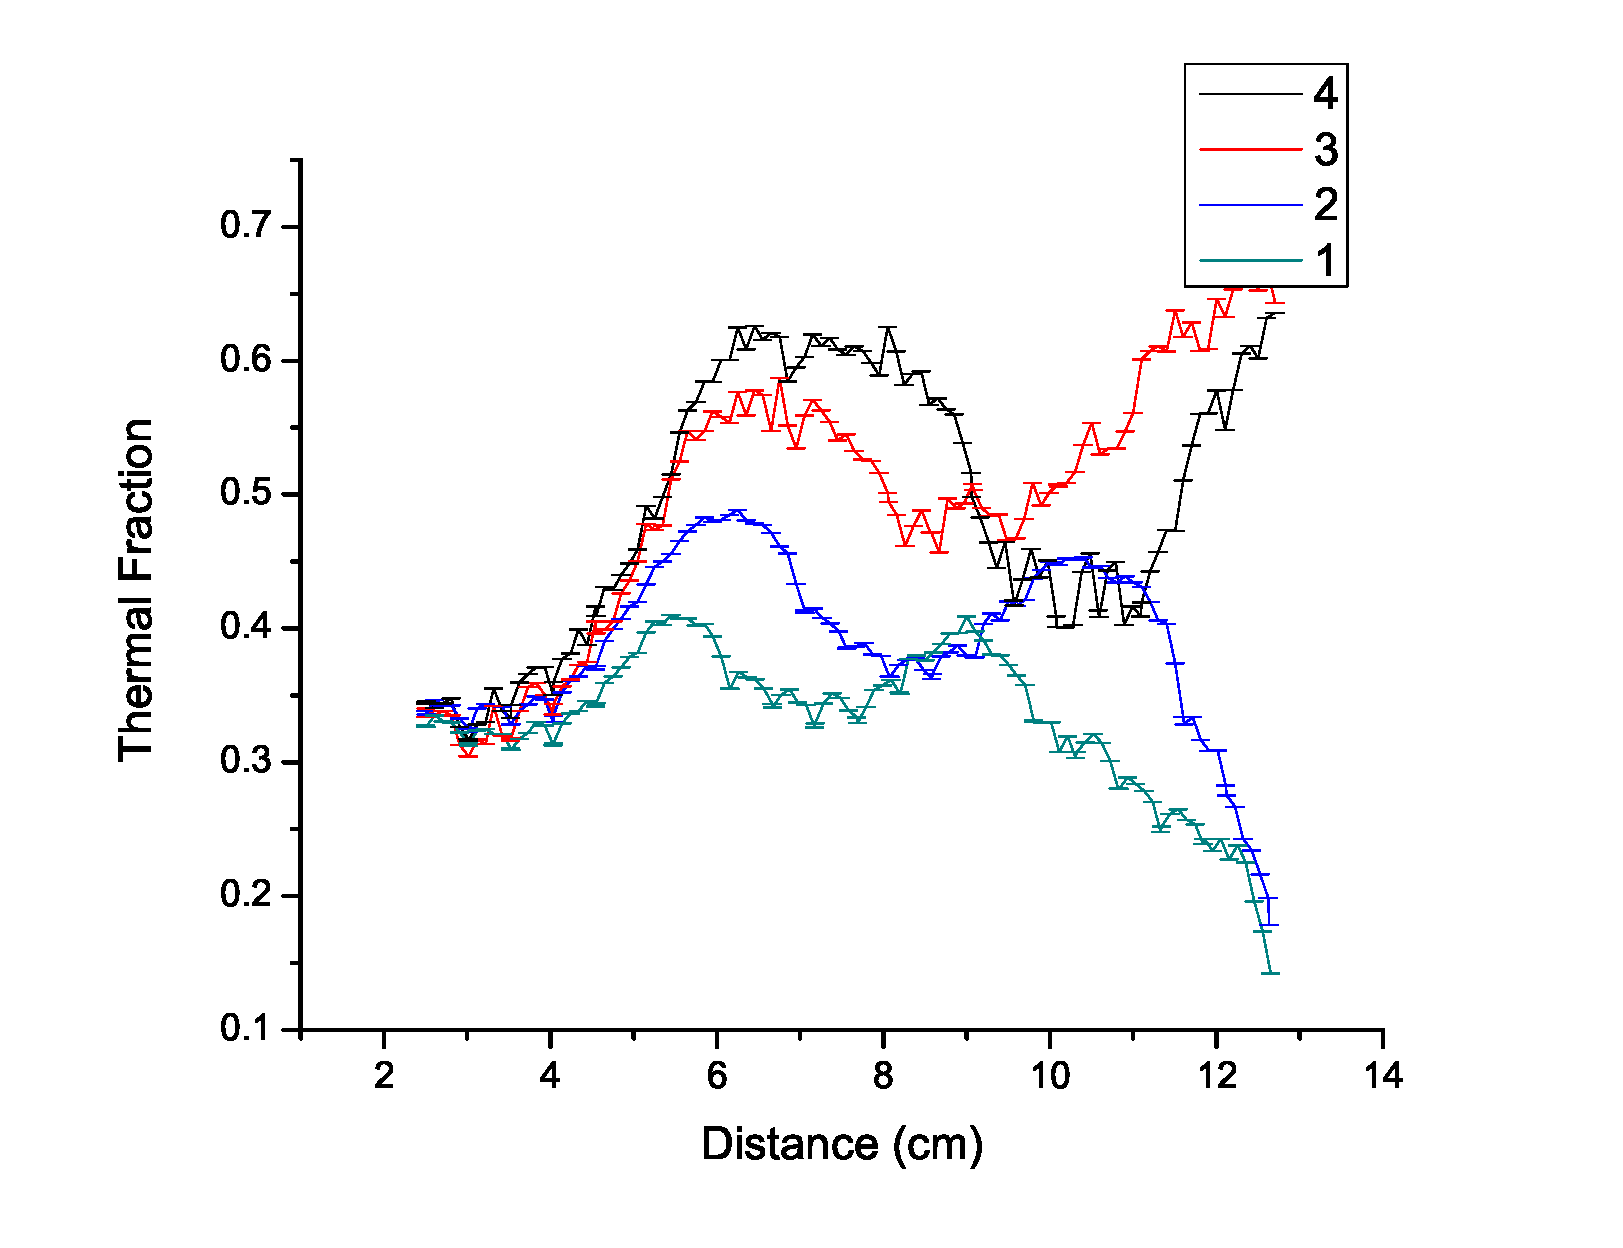
\includegraphics[width=\textwidth]{RPM8Opt_TF_5Assm.eps}
    \caption{5 Films per Assembly}
	\end{subfigure}%
	~
	\begin{subfigure}[b]{0.43\textwidth}
		\centering
		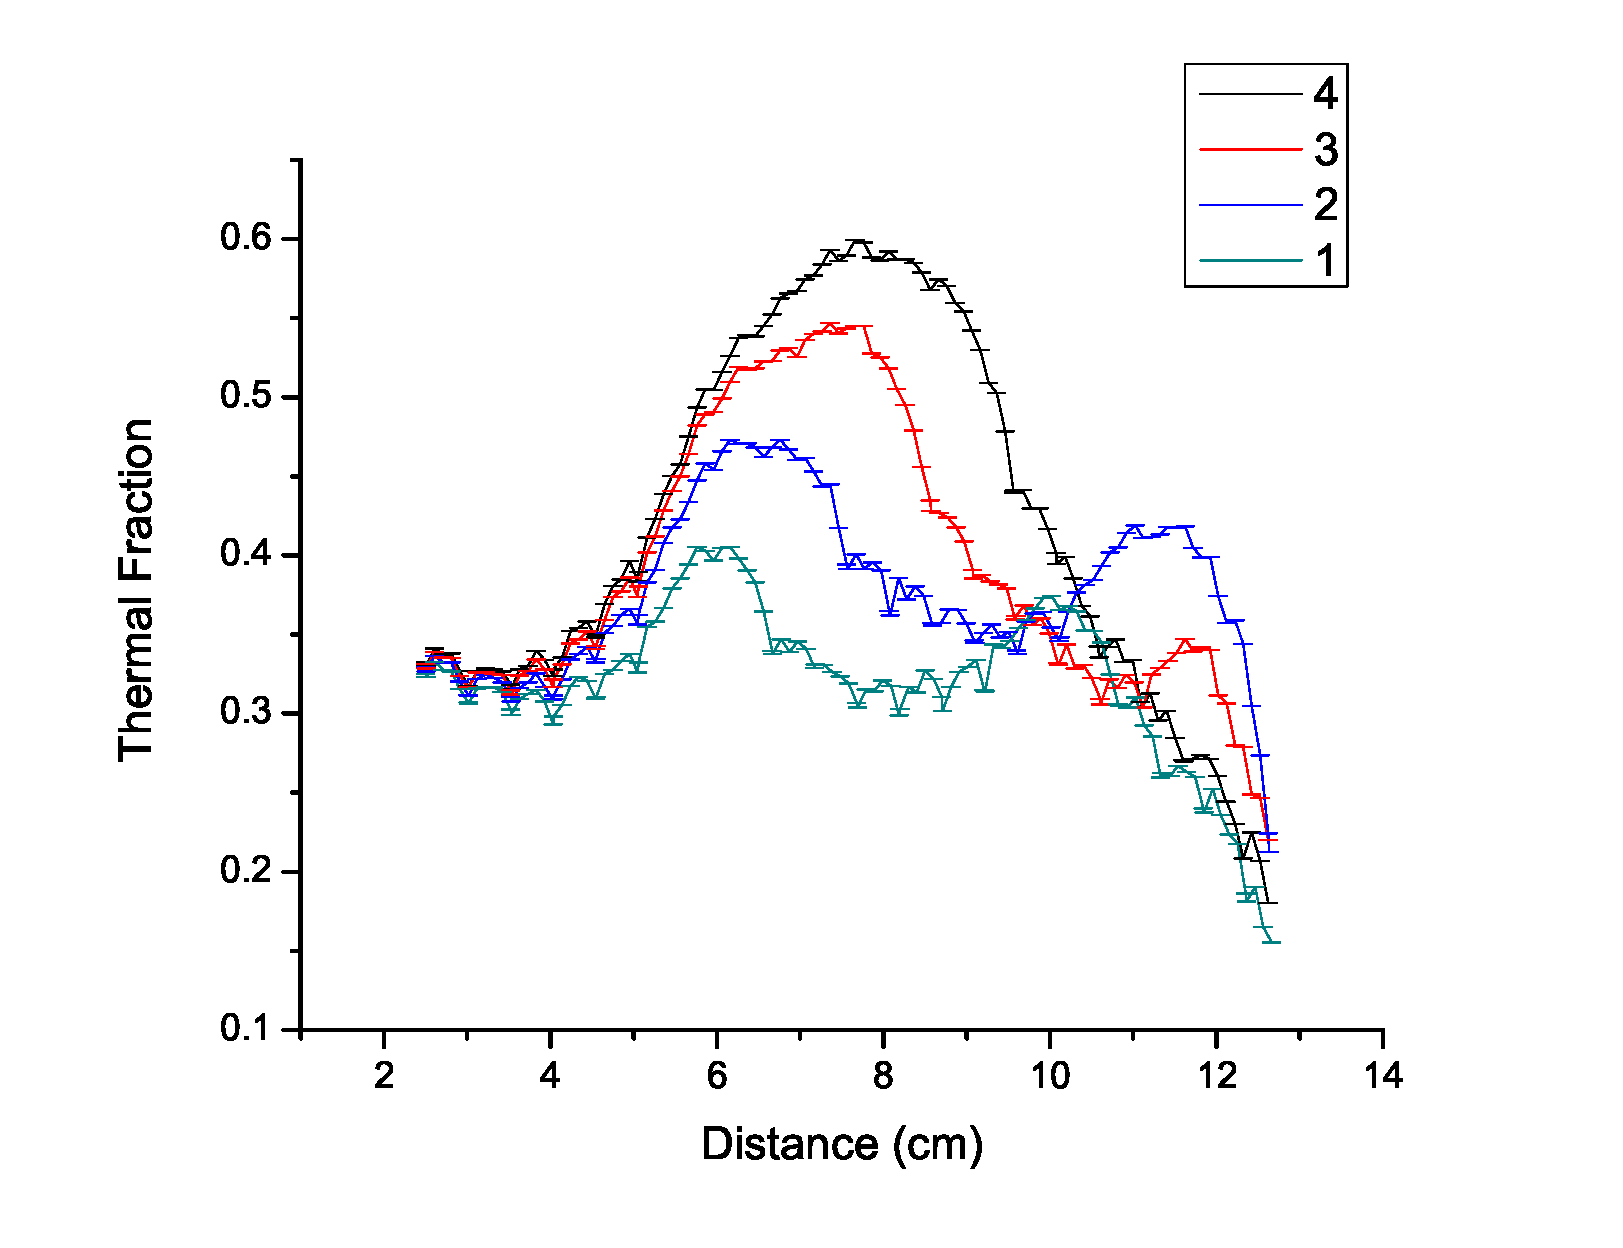
\includegraphics[width=\textwidth]{RPM8Opt_TF_6Assm.eps}
    \caption{6 Films per Assembly}
	\end{subfigure}

	\caption{Thermal Flux Profiles for Various Assemblies}
	\label{fig:ThermalFlux}
\end{figure}
\subsection{Optimzied Detector Configuration}
